% Documents setup
\documentclass[11pt]{book}

% fix for pandoc 1.14
\providecommand{\tightlist}{%
  \setlength{\itemsep}{0pt}\setlength{\parskip}{0pt}}

\usepackage{tabu} % https://tex.stackexchange.com/questions/50332/vertical-spacing-of-a-table-cell

% Location of the csas-style repository: adjust path as needed
\newcommand{\locRepo}{csas-style}

% Use the style file in the csas-style repository (res-doc.sty)
\usepackage{\locRepo/res-doc}

% header-includes from R markdown entry
\setcounter{section}{1}

% Headers and footers
\lhead{Draft working paper --- Do not cite or circulate}
% \lhead{}
\rhead{}
% \rfoot{DRAFT - DO NOT CITE}

%%%% Commands for title page etc %%%%%

% Publication year
\newcommand{\rdYear}{2020}

% Publication month
\newcommand{\rdMonth}{}

% Report number
\newcommand{\rdNumber}{nnn}

% Region
\newcommand{\rdRegion}{Pacific Region}

% Title
\newcommand{\rdTitle}{Update to the assessment of Pacific Cod (\emph{Gadus macrocephalus}) for Hecate Strait and Queen Charlotte Sound (Area 5ABCD), and West Coast Vancouver Island (Area 3CD) in 2020}

% Author names separated by commas and ', and' for the last author in the format 'M.H. Grinnell' (use \textsuperscript{n} for addresses)
\newcommand{\rdAuth}{Robyn E. Forrest\textsuperscript{1}, Sean C. Anderson\textsuperscript{1}, Chris J. Grandin\textsuperscript{1}}

% Author names reversed separated by commas in the format 'Grinnell, M.H.'
\newcommand{\rdAuthRev}{Forrest, R.E., Anderson, S.C., and Grandin, C.J.}

% Author addresses (use \textsuperscript{n})
\newcommand{\rdAuthAddy}{\textsuperscript{1}Pacific Biological Station\\
Fisheries and Oceans Canada, 3190 Hammond Bay Road\\
Nanaimo, British Columbia, V9T 6N7, Canada\\}

\newcommand{\citationOtherLanguage}{}

% Name of file with abstract and resume (see \abstract and \frenchabstract for requirements)
\newcommand{\rdAbstract}{\abstract{The status of two stocks of Pacific Cod (\emph{Gadus macrocephalus}) in Hecate Strait/Queen Charlotte Sound (Area 5ABCD) and West Coast Vancouver Island (Area 3CD) was updated from the 2018 assessment, using Bayesian delay-difference models and data streams updated to 2019. The models were fit to fishery-independent indices of abundance and standardized commercial catch-per-unit-effort (CPUE) indices, updated from the 2018 stock assessment.}}

%%%% End of title page commands %%%%%

% \pdfcompresslevel=5 % faster PNGs

\setcounter{section}{0}

\bibliographystyle{csas-style/res-doc}

\usepackage{amsmath}
\usepackage{bm}

% commands and environments needed by pandoc snippets
% extracted from the output of `pandoc -s`
%% Make R markdown code chunks work
\usepackage{array}
\usepackage{amssymb,amsmath}
\usepackage{color}
\usepackage{fancyvrb}
\DefineShortVerb[commandchars=\\\{\}]{\|}
\DefineVerbatimEnvironment{Highlighting}{Verbatim}{commandchars=\\\{\}}
% Add ',fontsize=\small' for more characters per line
\newenvironment{Shaded}{}{}
\newcommand{\KeywordTok}[1]{\textcolor[rgb]{0.00,0.44,0.13}{\textbf{{#1}}}}
\newcommand{\DataTypeTok}[1]{\textcolor[rgb]{0.56,0.13,0.00}{{#1}}}
\newcommand{\DecValTok}[1]{\textcolor[rgb]{0.25,0.63,0.44}{{#1}}}
\newcommand{\BaseNTok}[1]{\textcolor[rgb]{0.25,0.63,0.44}{{#1}}}
\newcommand{\FloatTok}[1]{\textcolor[rgb]{0.25,0.63,0.44}{{#1}}}
\newcommand{\CharTok}[1]{\textcolor[rgb]{0.25,0.44,0.63}{{#1}}}
\newcommand{\StringTok}[1]{\textcolor[rgb]{0.25,0.44,0.63}{{#1}}}
\newcommand{\CommentTok}[1]{\textcolor[rgb]{0.38,0.63,0.69}{\textit{{#1}}}}
\newcommand{\OtherTok}[1]{\textcolor[rgb]{0.00,0.44,0.13}{{#1}}}
\newcommand{\AlertTok}[1]{\textcolor[rgb]{1.00,0.00,0.00}{\textbf{{#1}}}}
\newcommand{\FunctionTok}[1]{\textcolor[rgb]{0.02,0.16,0.49}{{#1}}}
\newcommand{\RegionMarkerTok}[1]{{#1}}
\newcommand{\ErrorTok}[1]{\textcolor[rgb]{1.00,0.00,0.00}{\textbf{{#1}}}}
\newcommand{\NormalTok}[1]{{#1}}
\newcommand{\OperatorTok}[1]{\textcolor[rgb]{0.00,0.44,0.13}{\textbf{{#1}}}}
\newcommand{\BuiltInTok}[1]{\textcolor[rgb]{0.00,0.44,0.13}{\textbf{{#1}}}}
\newcommand{\ControlFlowTok}[1]{\textcolor[rgb]{0.00,0.44,0.13}{\textbf{{#1}}}}

%Defines cslreferences environment
%Required by pandoc 2.8
%Copied from https://github.com/rstudio/rmarkdown/issues/1649

\DeclareGraphicsExtensions{.png,.pdf}
\begin{document}

\frontmatter
\begin{verbatim}
#> create.rdata.file: RData file found in C:/GitHub/pacific-cod-2020/models/0_1a_5ABCD_BASE_2020
#> 
#> create.rdata.file: RData file found in C:/GitHub/pacific-cod-2020/models/1_1a_3CD_BASE_2020
#> 
#> create.rdata.file: RData file found in C:/GitHub/pacific-cod-2020/models/0_1a_5ABCD_BASE_2020
#> 
#> create.rdata.file: RData file found in C:/GitHub/pacific-cod-2020/models/0_2d_5ABCD_rsoleq_1_1
#> 
#> create.rdata.file: RData file found in C:/GitHub/pacific-cod-2020/models/0_2e_5ABCD_q_cv06
#> 
#> create.rdata.file: RData file found in C:/GitHub/pacific-cod-2020/models/0_3a_5ABCD_Mprior_mean04_sd01
#> 
#> create.rdata.file: RData file found in C:/GitHub/pacific-cod-2020/models/0_5a_5ABCD_kage_3
#> 
#> create.rdata.file: RData file found in C:/GitHub/pacific-cod-2020/models/0_6b_5ABCD_sig015
#> 
#> create.rdata.file: RData file found in C:/GitHub/pacific-cod-2020/models/0_7b_5ABCD_sigW_015
#> 
#> create.rdata.file: RData file found in C:/GitHub/pacific-cod-2020/models/1_1a_3CD_BASE_2020
#> 
#> create.rdata.file: RData file found in C:/GitHub/pacific-cod-2020/models/1_2d_3CD_q_1
#> 
#> create.rdata.file: RData file found in C:/GitHub/pacific-cod-2020/models/1_2e_3CD_q_cv06
#> 
#> create.rdata.file: RData file found in C:/GitHub/pacific-cod-2020/models/1_3a_3CD_Mprior_mean04_sd01
#> 
#> create.rdata.file: RData file found in C:/GitHub/pacific-cod-2020/models/1_5a_3CD_kage3
#> 
#> create.rdata.file: RData file found in C:/GitHub/pacific-cod-2020/models/1_6b_3CD_sig015
#> 
#> create.rdata.file: RData file found in C:/GitHub/pacific-cod-2020/models/1_7b_3CD_sigW015
\end{verbatim}
\clearpage

\hypertarget{introduction}{%
\section{Introduction}\label{introduction}}

The last Pacific Cod assessment was conducted in 2018 (Forrest et al. \protect\hyperlink{ref-forrest2020}{2020} p. @dfo2019). Separarat assessments were provided for stocks in Area 3CD and Area 5ABCD (Figure~\ref{fig:fig-map}). The assessment models were delay-difference models, fit to survey indices, commercial catch-per-unit-effort (CPUE), commercial catch data and commercial annual mean weights.

\emph{TODO: background on the reason we did this. Refer to SAR, wherever possible. Add SAR to refs}
\begin{figure}[htb]

{\centering \pdftooltip{\includegraphics[width=6in]{knitr-figs/fig-wcvi-index-3cd-1}}{Figure \ref{fig:fig-wcvi-index-3cd}} 

}

\caption{West Coast Vancouver Island Synoptic Survey estimates, centred by geometric mean}\label{fig:fig-wcvi-index-3cd}
\end{figure}
\hypertarget{summary}{%
\section{Summary}\label{summary}}

\emph{TODO: Put main figures here and discussion of each.}

3CD index 3CD CPUE 3CD Biomass

5ABCD index 5ABCD CPUE 5ABCD Biomass

A more complete set of tables and figures is provided in the following sections.

\hypertarget{full-results}{%
\section{Full results}\label{full-results}}

Briefly discuss each Table and Fig \ldots{} update text from 2018 assessment

\clearpage

\hypertarget{figures}{%
\section{FIGURES}\label{figures}}
\begin{figure}[htb]

{\centering \pdftooltip{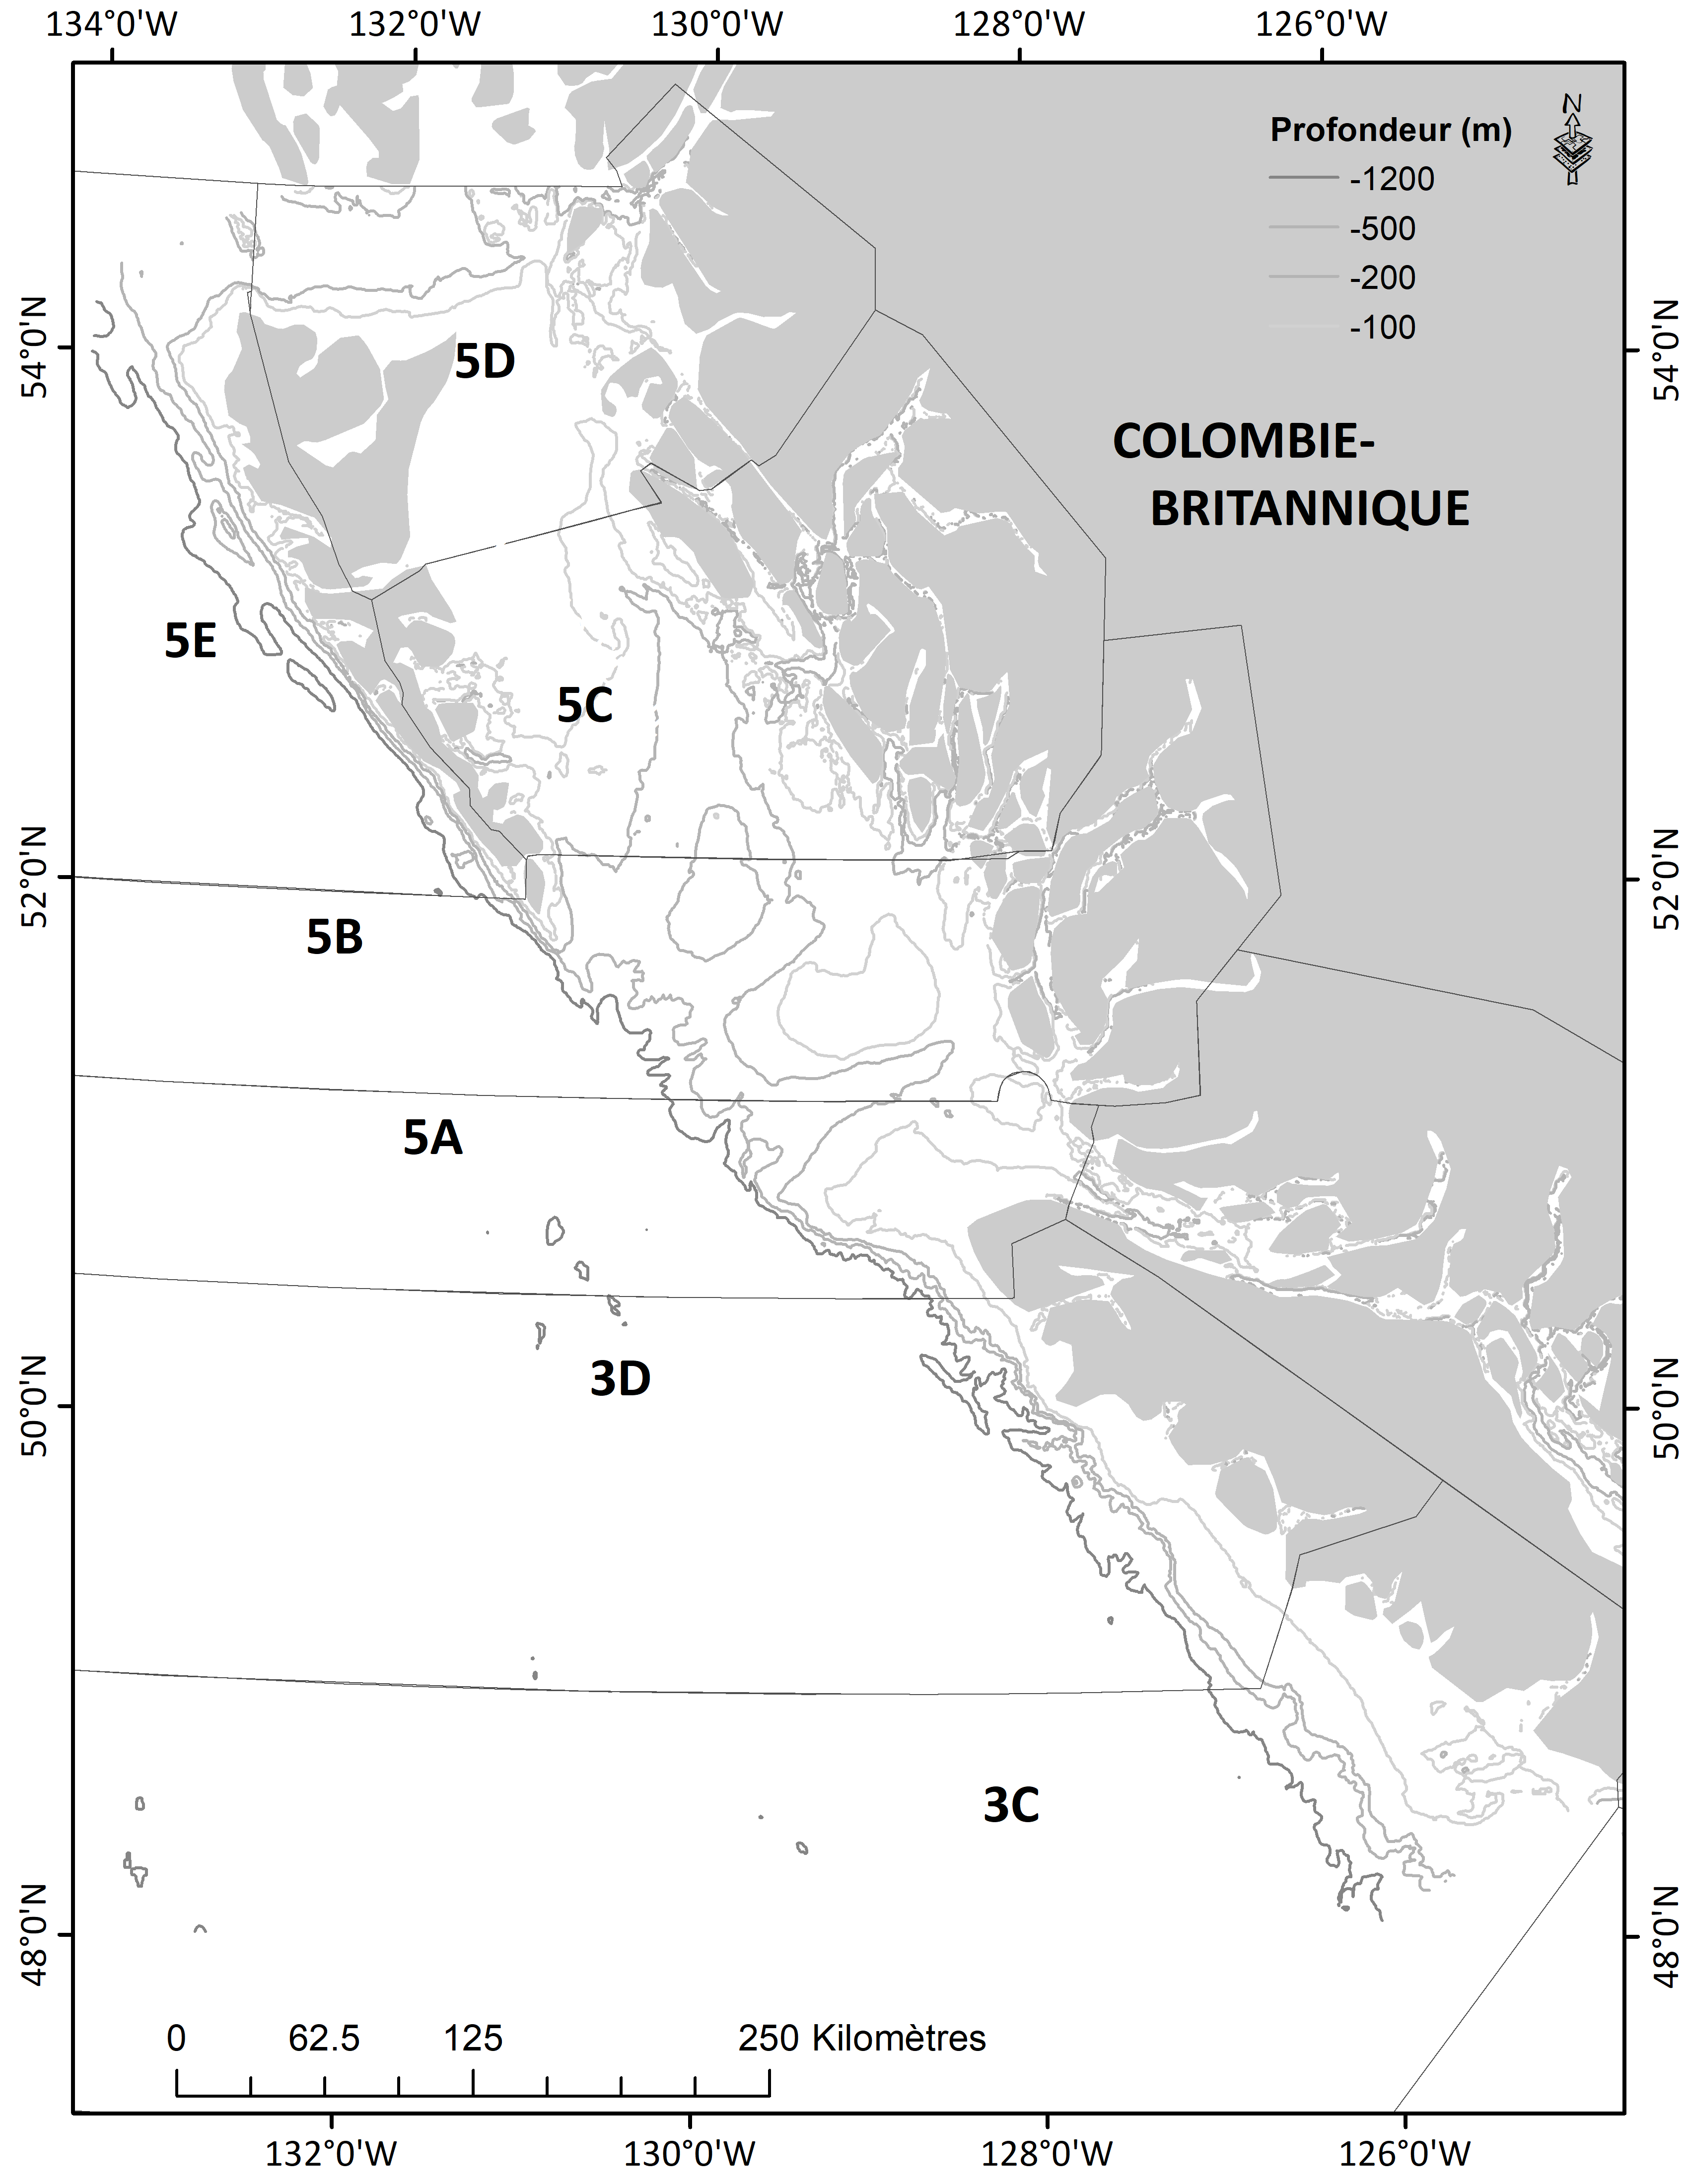
\includegraphics[width=4in]{C:/GitHub/pacific-cod-2020/report/figure/Pcod_3CD5ABCDE_Pic}}{Figure \ref{fig:fig-map}} 

}

\caption{Map of the management areas 5AB (Queen Charlotte Sound), 5CD (Hecate Strait), and 3CD (West Coast Vancouver Island).}\label{fig:fig-map}
\end{figure}
\clearpage

\hypertarget{catch-area-5abcd}{%
\subsection{CATCH: AREA 5ABCD}\label{catch-area-5abcd}}
\begin{figure}[htb]

{\centering \pdftooltip{\includegraphics[width=6in]{knitr-figs/fig-catch-5abcd-1}}{Figure \ref{fig:fig-catch-5abcd}} 

}

\caption{Catch for Area 5ABCD. Canadian catch includes at-sea releases.}\label{fig:fig-catch-5abcd}
\end{figure}
\begin{figure}[htb]

{\centering \pdftooltip{\includegraphics[width=6in]{knitr-figs/fig-discards-5abcd-1}}{Figure \ref{fig:fig-discards-5abcd}} 

}

\caption{Estimated at-sea releases of Pacific Cod by bottom trawlers for Area 5ABCD.}\label{fig:fig-discards-5abcd}
\end{figure}
\begin{figure}[htb]

{\centering \pdftooltip{\includegraphics[width=6in]{knitr-figs/fig-catch-5ab-1}}{Figure \ref{fig:fig-catch-5ab}} 

}

\caption{Catch for Area 5AB. Canadian catch includes at-sea releases.}\label{fig:fig-catch-5ab}
\end{figure}
\begin{figure}[htb]

{\centering \pdftooltip{\includegraphics[width=6in]{knitr-figs/fig-discards-5ab-1}}{Figure \ref{fig:fig-discards-5ab}} 

}

\caption{Estimated at-sea releases of Pacific Cod by bottom trawlers for Area 5AB.}\label{fig:fig-discards-5ab}
\end{figure}
\begin{figure}[htb]

{\centering \pdftooltip{\includegraphics[width=6in]{knitr-figs/fig-catch-5cd-1}}{Figure \ref{fig:fig-catch-5cd}} 

}

\caption{Catch for Area 5CD. Canadian catch includes at-sea releases.}\label{fig:fig-catch-5cd}
\end{figure}
\begin{figure}[htb]

{\centering \pdftooltip{\includegraphics[width=6in]{knitr-figs/fig-discards-5cd-1}}{Figure \ref{fig:fig-discards-5cd}} 

}

\caption{Estimated at-sea releases of Pacific Cod by bottom trawlers for Area 5CD.}\label{fig:fig-discards-5cd}
\end{figure}
\clearpage

\hypertarget{catch-area-3cd}{%
\subsection{CATCH: AREA 3CD}\label{catch-area-3cd}}
\begin{figure}[htb]

{\centering \pdftooltip{\includegraphics[width=6in]{knitr-figs/fig-catch-3cd-1}}{Figure \ref{fig:fig-catch-3cd}} 

}

\caption{Catch for Area 3CD. Canadian catch includes at-sea releases.}\label{fig:fig-catch-3cd}
\end{figure}
\begin{figure}[htb]

{\centering \pdftooltip{\includegraphics[width=6in]{knitr-figs/fig-discards-3cd-1}}{Figure \ref{fig:fig-discards-3cd}} 

}

\caption{Estimated at-sea releases of Pacific Cod by bottom trawlers for Area 3CD.}\label{fig:fig-discards-3cd}
\end{figure}
\clearpage

\hypertarget{prior-probability-distributions}{%
\subsection{PRIOR PROBABILITY DISTRIBUTIONS}\label{prior-probability-distributions}}
\begin{figure}[htb]

{\centering \pdftooltip{\includegraphics[width=6in]{knitr-figs/fig-base-mcmc-priors-5abcd-1}}{Figure \ref{fig:fig-base-mcmc-priors-5abcd}} 

}

\caption{Prior probability distributions used in the Area 5ABCD reference model. $q_1$ = Hecate Strait Assemblage survey, $q_2$ = Queen Charlotte Sound Synoptic Survey, $q_3$ = Hecate Strait Synoptic Survey, $q_4$ = Commercial CPUE pre-1996, and $q_5$ = Commercial CPUE post-1995.}\label{fig:fig-base-mcmc-priors-5abcd}
\end{figure}
\begin{figure}[htb]

{\centering \pdftooltip{\includegraphics[width=6in]{knitr-figs/fig-base-mcmc-priors-3cd-1}}{Figure \ref{fig:fig-base-mcmc-priors-3cd}} 

}

\caption{Prior probability distributions used in the Area 3CD reference model. $q_1$ = West Coast Vancouver Island Synoptic Survey, $q_2$ = Commercial CPUE pre-1996, $q_3$ = Commercial CPUE post-1995, and $q_4$ = NMFS Triennial Survey (Canadian portion).}\label{fig:fig-base-mcmc-priors-3cd}
\end{figure}
\clearpage

\hypertarget{model-results-area-5abcd}{%
\subsection{MODEL RESULTS: AREA 5ABCD}\label{model-results-area-5abcd}}
\begin{figure}[htb]

{\centering \pdftooltip{\includegraphics[width=6in]{knitr-figs/fig-base-mcmc-trace-5abcd-1}}{Figure \ref{fig:fig-base-mcmc-trace-5abcd}} 

}

\caption{Traceplots of posterior samples for the Area 5ABCD reference model. $q_1$ = Hecate Strait Assemblage survey, $q_2$ = Queen Charlotte Sound Synoptic Survey, $q_3$ = Hecate Strait Synoptic Survey, $q_4$ = Commercial CPUE pre-1996, and $q_5$ = Commercial CPUE post-1995.}\label{fig:fig-base-mcmc-trace-5abcd}
\end{figure}
\begin{figure}[htb]

{\centering \pdftooltip{\includegraphics[width=6in]{knitr-figs/fig-base-mcmc-autocor-5abcd-1}}{Figure \ref{fig:fig-base-mcmc-autocor-5abcd}} 

}

\caption{Autocorrelation plots for the Area 5ABCD reference model. $q_1$ = Hecate Strait Assemblage survey, $q_2$ = Queen Charlotte Sound Synoptic Survey, $q_3$ = Hecate Strait Synoptic Survey, $q_4$ = Commercial CPUE pre-1996, and $q_5$ = Commercial CPUE post-1995.}\label{fig:fig-base-mcmc-autocor-5abcd}
\end{figure}
\begin{figure}[htb]

{\centering \pdftooltip{\includegraphics[width=6in]{knitr-figs/fig-base-index-fits-5abcd-1}}{Figure \ref{fig:fig-base-index-fits-5abcd}} 

}

\caption{MPD fits to observed indices of abundance (points) for the Area 5ABCD reference model from: (a) the Hecate Strait Assemblage survey, (b) the Queen Charlotte Sound Synoptic Survey, (c) the Hecate Strait Synoptic Survey, (d) the Commercial CPUE pre-1996, and (e) the Commercial CPUE post-1995. For clarity, only MPD results are shown}\label{fig:fig-base-index-fits-5abcd}
\end{figure}
\begin{figure}[htb]

{\centering \pdftooltip{\includegraphics[width=6in]{knitr-figs/fig-base-mean-weight-5abcd-1}}{Figure \ref{fig:fig-base-mean-weight-5abcd}} 

}

\caption{MPD fit to the mean weight data for Area 5ABCD reference model. For clarity, only MPD results are shown}\label{fig:fig-base-mean-weight-5abcd}
\end{figure}
\begin{figure}[htb]

{\centering \pdftooltip{\includegraphics[width=6in]{knitr-figs/fig-base-catch-fit-5abcd-1}}{Figure \ref{fig:fig-base-catch-fit-5abcd}} 

}

\caption{MPD fit to the catch data for Area 5ABCD reference model. For clarity, only MPD results are shown}\label{fig:fig-base-catch-fit-5abcd}
\end{figure}

\begin{figure}[htb]

{\centering \pdftooltip{\includegraphics[width=6in]{knitr-figs/fig-base-mcmc-priors-posts-5abcd-1}}{Figure \ref{fig:fig-base-mcmc-priors-posts-5abcd}} 

}

\caption{Histograms of posterior samples with prior probability distributions (lines) used in the Area 5ABCD reference model. MPD estimate shown as vertical dashed line. Note that both the Queen Charlotte Sound and Hecate Strait Synoptic Surveys used normal prior distributions on \(ln(q)\), see Figure~\ref{fig:fig-base-mcmc-priors-5abcd} for full distribution. $q_1$ = Hecate Strait Assemblage survey, $q_2$ = Queen Charlotte Sound Synoptic Survey, $q_3$ = Hecate Strait Synoptic Survey, $q_4$ = Commercial CPUE pre-1996, and $q_5$ = Commercial CPUE post-1995.}\label{fig:fig-base-mcmc-priors-posts-5abcd}
\end{figure}
\begin{figure}[htb]

{\centering \pdftooltip{\includegraphics[width=6in]{knitr-figs/fig-base-mcmc-pairs-5abcd-1}}{Figure \ref{fig:fig-base-mcmc-pairs-5abcd}} 

}

\caption{Pairs plots of posterior samples for the Area 5ABCD reference model. $\bar{R} = R_{Avg}$, $q_1$ = Hecate Strait Assemblage survey, $q_2$ = Queen Charlotte Sound Synoptic Survey, $q_3$ = Hecate Strait Synoptic Survey, $q_4$ = Commercial CPUE pre-1996, and $q_5$ = Commercial CPUE post-1995.}\label{fig:fig-base-mcmc-pairs-5abcd}
\end{figure}
\begin{figure}[htb]

{\centering \pdftooltip{\includegraphics[width=6in]{knitr-figs/fig-base-biomass-5abcd-1}}{Figure \ref{fig:fig-base-biomass-5abcd}} 

}

\caption{Posterior estimated biomass for the Reference Model, Area 5ABCD.  The green dashed line shows the median Upper Stock Reference (USR) which is the mean biomass estimate for the years 1956--2004. The red dashed line shows the median Limit Reference Point (LRP) which is the lowest estimated biomass agreed to be an undesirable state to avoid, in this case it is the biomass estimate for 2000.}\label{fig:fig-base-biomass-5abcd}
\end{figure}
\begin{figure}[htb]

{\centering \pdftooltip{\includegraphics[width=6in]{knitr-figs/fig-base-depl-5abcd-1}}{Figure \ref{fig:fig-base-depl-5abcd}} 

}

\caption{Relative biomass for the Reference Model, Area 5ABCD.}\label{fig:fig-base-depl-5abcd}
\end{figure}
\begin{figure}[htb]

{\centering \pdftooltip{\includegraphics[width=6in]{knitr-figs/fig-base-recr-5abcd-1}}{Figure \ref{fig:fig-base-recr-5abcd}} 

}

\caption{Recruitment (a) and recruitment deviations (b) for the Reference Model, Area 5ABCD.  The green dashed line shows the mean of the MCMC posterior medians, the blue dashed line shows the median of the MCMC posterior medians.}\label{fig:fig-base-recr-5abcd}
\end{figure}
\begin{figure}[htb]

{\centering \pdftooltip{\includegraphics[width=6in]{knitr-figs/fig-base-f-5abcd-1}}{Figure \ref{fig:fig-base-f-5abcd}} 

}

\caption{Fishing mortality for the Reference Model, Area 5ABCD.}\label{fig:fig-base-f-5abcd}
\end{figure}
\clearpage

\hypertarget{model-results-area-3cd}{%
\subsection{MODEL RESULTS: AREA 3CD}\label{model-results-area-3cd}}
\begin{figure}[htb]

{\centering \pdftooltip{\includegraphics[width=6in]{knitr-figs/fig-base-mcmc-trace-3cd-1}}{Figure \ref{fig:fig-base-mcmc-trace-3cd}} 

}

\caption{Traceplots of posterior samples for the Area 3CD reference model. $q_1$ = West Coast Vancouver Island Synoptic Survey, $q_2$ = Commercial CPUE pre-1996, $q_3$ = Commercial CPUE post-1995, and $q_4$ = NMFS Triennial Survey (Canadian portion).}\label{fig:fig-base-mcmc-trace-3cd}
\end{figure}
\begin{figure}[htb]

{\centering \pdftooltip{\includegraphics[width=6in]{knitr-figs/fig-base-mcmc-autocor-3cd-1}}{Figure \ref{fig:fig-base-mcmc-autocor-3cd}} 

}

\caption{Autocorrelation plots for the Area 3CD reference model. $q_1$ = West Coast Vancouver Island Synoptic Survey, $q_2$ = Commercial CPUE pre-1996, $q_3$ = Commercial CPUE post-1995, and $q_4$ = NMFS Triennial Survey (Canadian portion).}\label{fig:fig-base-mcmc-autocor-3cd}
\end{figure}
\begin{figure}[htb]

{\centering \pdftooltip{\includegraphics[width=6in]{knitr-figs/fig-base-index-fits-3cd-1}}{Figure \ref{fig:fig-base-index-fits-3cd}} 

}

\caption{MPD fits to observed indices of abundance (points) for the Area 3CD reference model from: (a) the West Coast Vancouver Island Synoptic Survey, (b) the Commercial CPUE pre-1996, (c) the Commercial CPUE post-1995, and (d) the NMFS Triennial Survey (Canadian portion).}\label{fig:fig-base-index-fits-3cd}
\end{figure}
\begin{figure}[htb]

{\centering \pdftooltip{\includegraphics[width=6in]{knitr-figs/fig-base-mean-weight-3cd-1}}{Figure \ref{fig:fig-base-mean-weight-3cd}} 

}

\caption{MPD fit to the mean weight data for Area 3CD reference model.}\label{fig:fig-base-mean-weight-3cd}
\end{figure}
\begin{figure}[htb]

{\centering \pdftooltip{\includegraphics[width=6in]{knitr-figs/fig-base-catch-fit-3cd-1}}{Figure \ref{fig:fig-base-catch-fit-3cd}} 

}

\caption{MPD fit to the catch data for Area 3CD reference model.}\label{fig:fig-base-catch-fit-3cd}
\end{figure}

\begin{figure}[htb]

{\centering \pdftooltip{\includegraphics[width=6in]{knitr-figs/fig-base-mcmc-priors-posts-3cd-1}}{Figure \ref{fig:fig-base-mcmc-priors-posts-3cd}} 

}

\caption{Histograms of posterior samples with prior probability distributions (lines) used in the Area 3CD reference model. MPD estimate shown as vertical dashed line. Note that the West Coast Vancouver Island Synoptic Survey used a normal prior distribution on \(ln(q)\), see Figure~\ref{fig:fig-base-mcmc-priors-3cd} for full distribution. $q_1$ = West Coast Vancouver Island Synoptic Survey, $q_2$ = Commercial CPUE pre-1996, $q_3$ = Commercial CPUE post-1995, and $q_4$ = NMFS Triennial Survey (Canadian portion).}\label{fig:fig-base-mcmc-priors-posts-3cd}
\end{figure}
\begin{figure}[htb]

{\centering \pdftooltip{\includegraphics[width=6in]{knitr-figs/fig-base-mcmc-pairs-3cd-1}}{Figure \ref{fig:fig-base-mcmc-pairs-3cd}} 

}

\caption{Pairs plots of posterior samples for the Area 3CD reference model. $q_1$ = West Coast Vancouver Island Synoptic Survey, $q_2$ = Commercial CPUE pre-1996, $q_3$ = Commercial CPUE post-1995, and $q_4$ = NMFS Triennial Survey (Canadian portion).}\label{fig:fig-base-mcmc-pairs-3cd}
\end{figure}
\begin{figure}[htb]

{\centering \pdftooltip{\includegraphics[width=6in]{knitr-figs/fig-base-biomass-3cd-1}}{Figure \ref{fig:fig-base-biomass-3cd}} 

}

\caption{Posterior estimated biomass for the Reference Model, Area 3CD. The green dashed line shows the median Upper Stock Reference (USR) which is the mean biomass estimate for the years 1956--2004. The red dashed line shows the median Limit Reference Point (LRP) which is the lowest estimated biomass agreed to be an undesirable state to avoid, in this case it is the biomass estimate for 1986.}\label{fig:fig-base-biomass-3cd}
\end{figure}
\begin{figure}[htb]

{\centering \pdftooltip{\includegraphics[width=6in]{knitr-figs/fig-base-depl-3cd-1}}{Figure \ref{fig:fig-base-depl-3cd}} 

}

\caption{Relative biomass for the Reference Model, Area 3CD.}\label{fig:fig-base-depl-3cd}
\end{figure}
\begin{figure}[htb]

{\centering \pdftooltip{\includegraphics[width=6in]{knitr-figs/fig-base-recr-3cd-1}}{Figure \ref{fig:fig-base-recr-3cd}} 

}

\caption{Recruitment (a) and recruitment deviations (b) for the Reference Model, Area 3CD.  The green dashed line shows the mean of the MCMC posterior medians, the blue dashed line shows the median of the MCMC posterior medians.}\label{fig:fig-base-recr-3cd}
\end{figure}
\begin{figure}[htb]

{\centering \pdftooltip{\includegraphics[width=6in]{knitr-figs/fig-base-f-3cd-1}}{Figure \ref{fig:fig-base-f-3cd}} 

}

\caption{Fishing mortality for the Reference Model, Area 3CD.}\label{fig:fig-base-f-3cd}
\end{figure}
\clearpage
\begin{figure}[htb]

{\centering \pdftooltip{\includegraphics[width=6in]{knitr-figs/fig-model-average-biomass-comp-5abcd-1}}{Figure \ref{fig:fig-model-average-biomass-comp-5abcd}} 

}

\caption{Posterior estimates of biomass for the model-averaged set for Area 5ABCD. The green dashed line shows the median Upper Stock Reference (USR) which is the mean biomass estimate for the years 1956--2004. The red dashed line shows the median Limit Reference Point (LRP) which is the lowest estimated biomass agreed to be an undesirable state to avoid, in this case it is the biomass estimate for 2000.}\label{fig:fig-model-average-biomass-comp-5abcd}
\end{figure}
\begin{figure}[htb]

{\centering \pdftooltip{\includegraphics[width=6in]{knitr-figs/fig-model-average-biomass-5abcd-1}}{Figure \ref{fig:fig-model-average-biomass-5abcd}} 

}

\caption{Combined posterior biomass for the averaged models, Area 5ABCD. The green dashed line shows the median Upper Stock Reference (USR) which is the mean biomass estimate for the years 1956--2004. The red dashed line shows the median Limit Reference Point (LRP) which is the lowest estimated biomass agreed to be an undesirable state to avoid, in this case it is the biomass estimate for 2000.}\label{fig:fig-model-average-biomass-5abcd}
\end{figure}
\clearpage
\begin{figure}[htb]

{\centering \pdftooltip{\includegraphics[width=6in]{knitr-figs/fig-model-average-biomass-5abcd-proj-1}}{Figure \ref{fig:fig-model-average-biomass-5abcd-proj}} 

}

\caption{Combined posterior estimates of biomass for the model-averaged set for Area 5ABCD with projections (to the end of 2019).  The upper horizontal green dashed line shows the median Upper Stock Reference (USR) which is the mean biomass estimate for the years 1956--2004. The lower horizontal red dashed line shows the median Limit Reference Point (LRP) which is the lowest estimated biomass agreed to be an undesirable state to avoid, in this case it is the biomass estimate for 2000. The coloured regions to the right of the vertical line represent projections based on various TACs. The line represents the posterior median and the shaded region represents the 95\% credible interval. For clarity, years before 2010 are removed.}\label{fig:fig-model-average-biomass-5abcd-proj}
\end{figure}
\clearpage
\begin{figure}[htb]

{\centering \pdftooltip{\includegraphics[width=6in]{knitr-figs/fig-model-average-biomass-comp-3cd-1}}{Figure \ref{fig:fig-model-average-biomass-comp-3cd}} 

}

\caption{Posterior estimates of biomass for the model-averaged set for Area 3CD. The green dashed line shows the median Upper Stock Reference (USR) which is the mean biomass estimate for the years 1956--2004. The red dashed line shows the median Limit Reference Point (LRP) which is the lowest estimated biomass agreed to be an undesirable state to avoid, in this case it is the biomass estimate for 1986.}\label{fig:fig-model-average-biomass-comp-3cd}
\end{figure}
\clearpage
\begin{figure}[htb]

{\centering \pdftooltip{\includegraphics[width=6in]{knitr-figs/fig-model-average-biomass-3cd-1}}{Figure \ref{fig:fig-model-average-biomass-3cd}} 

}

\caption{Combined posterior biomass for the model-averaged set for Area 3CD.  The green dashed line shows the median Upper Stock Reference (USR) which is the mean biomass estimate for the years 1956--2004. The red dashed line shows the median Limit Reference Point (LRP) which is the lowest estimated biomass agreed to be an undesirable state to avoid, in this case it is the biomass estimate for 1986.}\label{fig:fig-model-average-biomass-3cd}
\end{figure}
\clearpage
\begin{figure}[htb]

{\centering \pdftooltip{\includegraphics[width=6in]{knitr-figs/fig-model-average-biomass-3cd-proj-1}}{Figure \ref{fig:fig-model-average-biomass-3cd-proj}} 

}

\caption{Combined posterior estimates of biomass for the model-averaged set for Area 3CD with projections (to the end of 2019).  The upper horizontal green dashed line shows the median Upper Stock Reference (USR) which is the mean biomass estimate for the years 1956--2004. The lower horizontal red dashed line shows the median Limit Reference Point (LRP) which is the lowest estimated biomass agreed to be an undesirable state to avoid, in this case it is the biomass estimate for 2000. The coloured regions to the right of the vertical line represent projections based on various TACs. The line represents the posterior median and the shaded region represents the 95\% credible interval.For clarity, years before 2010 are removed.}\label{fig:fig-model-average-biomass-3cd-proj}
\end{figure}
\clearpage

\hypertarget{references}{%
\section*{REFERENCES}\label{references}}
\phantomsection
\addcontentsline{toc}{section}{REFERENCES}
% This manually sets the header for this unnumbered chapter.
\noindent
\vspace{-2em}
\setlength{\parindent}{-0.2in}
\setlength{\leftskip}{0.2in}
\setlength{\parskip}{8pt}

\hypertarget{refs}{}
\leavevmode\hypertarget{ref-dfo2019}{}%
DFO. 2019. Assessment of British Columbia Pacific Cod for Areas 3CD and 5ABCD in 2018. (Science Advisory Report 2019/008).

\leavevmode\hypertarget{ref-forrest2020}{}%
Forrest, R.E., Anderson, S.C., Grandin, C.J., and Starr, P.J. 2020. Assessment of Pacific Cod (\emph{Gadus macrocephalus}) for Hecate Strait and Queen Charlotte Sound (Area 5ABCD), and West Coast Vancouver Island (Area 3CD) in 2018. DFO Can. Sci. Advis. Sec. Res. Doc. 2020/nnn(Canadian Science Advisory Secretariat (CSAS) 2020/nnn): nnn.

\setlength{\parindent}{0in} \setlength{\leftskip}{0in} \setlength{\parskip}{4pt}

\markboth{References}{References}

\end{document}
